\documentclass[twoside,11pt]{report}

% Any additional packages needed should be included after jmlr2e.
% Note that jmlr2e.sty includes epsfig, amssymb, natbib and graphicx,
% and defines many common macros, such as 'proof' and 'example'.
%
% It also sets the bibliographystyle to plainnat; for more information on
% natbib citation styles, see the natbib documentation, a copy of which
% is archived at http://www.jmlr.org/format/natbib.pdf

\usepackage{jmlr2e}
% \usepackage[utf8]{inputenc}%
% \usepackage{tikz}
% \usepackage{cfr-lm}%
\usepackage[T1]{fontenc}%
\usepackage{physics}
\usepackage{amsmath}
% \usepackage{amssymb}
% \usepackage{graphicx}
% \usepackage[margin=3cm]{geometry}
% \usepackage{changepage}
\usepackage{fontspec}
\usepackage{minted}
\usepackage{tcolorbox}
\usepackage{lmodern}
\usepackage{xcolor}
\usepackage{lettrine}
% \usepackage{fontawesome}
\usemintedstyle{perldoc}
\hypersetup{colorlinks=false, pdfborder={0 0 0},  }
\usepackage{fancyhdr}
\usepackage{wrapfig}
\usepackage{adjustbox}
\usepackage{tikz}
% \usepackage{listofitems} % for \readlist to create arrays
\usepackage{caption}
\usepackage[toc,page,header]{appendix}


\newtcbox{\codebox}[1][black]{on line, arc=2pt,colback=#1!10!white,colframe=white, before upper={\rule[-3pt]{0pt}{10pt}},boxrule=1pt, boxsep=0pt,left=2pt,right=2pt,top=1pt,bottom=.5pt}
\newtcbox{\deloppg}[1][black]{on line, arc=2pt,colback=#1!10!white,colframe=white, before upper={\rule[-2pt]{0pt}{0pt}},boxrule=0pt, boxsep=0pt,left=.49\linewidth,right=.49\linewidth,top=4pt,bottom=3pt}


\newcommand\blfootnote[1]{ \begingroup \renewcommand\thefootnote{}\footnote{#1} \addtocounter{footnote}{-1} \endgroup }
% \definecolor{antwhite}{HTML}{323333}
\newcommand{\code}[3][]{\codebox{\mintinline[#1]{#2}{#3}}}



% \setmainfont{FreeSans}
% \setmainfont{SF Pro Display}
% \setmainfont{IBM Plex Sans}
% \setmainfont{TeX Gyre Heros}
% \setmainfont{Inter}
% \setmainfont{Iosevka Quasi}
% \setmainfont{DM Sans}

% \setmonofont{Iosevka Custom Extended}
% \setmonofont{JetBrainsMono Nerd Font}
\setmonofont[Scale=MatchLowercase]{DM Mono}





% Definitions of handy macros can go here

\newcommand{\dataset}{{\cal D}}
\newcommand{\fracpartial}[2]{\frac{\partial #1}{\partial  #2}}

% Heading arguments are {volume}{year}{pages}{submitted}{published}{author-full-names}

% \jmlrheading{1}{2000}{1-48}{4/00}{10/00}{https://github.com/bragewiseth/MachineLearningProjects}

% Short headings should be running head and authors last names

\ShortHeadings{\url{https://github.com/bragewiseth/MachineLearningProjects}}{\url{https://github.com/bragewiseth/MachineLearningProjects}}
\firstpageno{1}



\title{{\huge Project 3}}
\author{\name Brage W. \email bragewi@ifi.uio.no\\
    \name Felix C. H.  \email felixch@ifi.uio.no \\
\name Eirik B. J. \email eiribja@ifi.uio.no}
\date{\today}											% Date
\makeatletter






% \date{\today}

\usepackage{hyperref}
\begin{document}

%%%%%%%%%%%%%%%%%%%%%%%%%%%%%%%%%%%%%%%%%%%%%%%%%%%%%%%%%%%%%%%%%%%%%%%%%%%%%%%%%%%%%%%%%

\begin{titlepage}
    \centering
    \vspace*{0.5 cm}
    
\includegraphics[scale = 0.75]{uio.jpg}\\[1.0 cm]	% University Logo
    \textsc{\LARGE University of Oslo}\\[2.0 cm]	    % University Name
    \textsc{\Large FYS-STK3155}\\[0.5 cm]				% Course Code
    \rule{\linewidth}{0.2 mm} \\[0.4 cm]
    { \huge \bfseries \@title}\\
    \rule{\linewidth}{0.2 mm} \\[1.5 cm]

    \begin{minipage}{0.4\textwidth}
        \begin{flushleft} \normalsize
            Brage Wiseth\\
            Felix Cameren Heyerdahl\\
            Eirik Bjørnson Jahr\\
        \end{flushleft}
    \end{minipage}~
    \begin{minipage}{0.4\textwidth}
        \begin{flushright} \normalsize
            \textsc{
                bragewi@ifi.uio.no\\
                felixch@ifi.uio.no\\
                eiribja@ifi.uio.no\\
            }
        \end{flushright}

    \end{minipage}\\[2 cm]
    \@date\\
    \vspace*{25mm}
    \urlstyle{rm}
    \textsc{\url{https://github.com/bragewiseth/MachineLearningProjects}}







\end{titlepage}
\nocite{*}
% \maketitle
\newpage
\tableofcontents
\newpage




\begin{abstract}%   <- trailing '%' for backward compatibility of .sty file
    \lettrine{I}{}
    Lorem ipsum dolor sit amet, officia excepteur ex fugiat reprehenderit enim labore culpa sint ad nisi Lorem pariatur mollit ex esse exercitation amet. Nisi anim cupidatat excepteur officia. Reprehenderit nostrud nostrud ipsum Lorem est aliquip amet voluptate voluptate dolor minim nulla est proident. Nostrud officia pariatur ut officia. Sit irure elit esse ea nulla sunt ex occaecat reprehenderit commodo officia dolor Lorem duis laboris cupidatat officia voluptate. Culpa proident adipisicing id nulla nisi laboris ex in Lorem sunt duis officia eiusmod. Aliqua reprehenderit commodo ex non excepteur duis sunt velit enim. Voluptate laboris sint cupidatat ullamco ut ea consectetur et est culpa et culpa duis.
\end{abstract}
\begin{keywords}
    Regression, Classification, Neural Networks
\end{keywords}





\addcontentsline{toc}{section}{Introduction}
\section*{Introduction}

    Wave equation is a partial differential equation that describes the propagation of waves through a medium.
    blah blah blah
    


    \noindent
    The structure of this report is as follows: 
    \begin{itemize}
        \item In \hyperref[sec:logistic]{Section 2}, we introduce the logistic regression model.
        \item In \hyperref[sec:GD]{Section 3}, we discuss gradient descent and backpropagation, key techniques in 
            the optimization of machine learning models.
        \item In \hyperref[sec:NN]{Section 4}, we delve into the fundamentals of neural networks.
        \item \hyperref[sec:data]{Section 5} covers the data used in our experiments and analyses.
        \item \hyperref[sec:resultsdiscussion]{Section 6} presents our results and provides a discussion on their 
            implications.
        \item \hyperref[sec:conclusion]{Section 7} concludes the report, summarizing key findings and insights.
        \item \hyperref[app:appendixA]{Appendix A} explores regression using neural networks.
        \item \hyperref[app:appendixB]{Appendix B} investigates the universal approximation theorem and its applications.
    \end{itemize}




\section{Wave Equation}
\label{sec:wave}

    The wave equation is a partial differential equation that describes the propagation of waves through a medium.
    It is given by
    \begin{equation}
        \frac{\partial^2 u}{\partial t^2} = c^2 \frac{\partial^2 u}{\partial x^2},
    \end{equation}
    where $u(x,t)$ is the displacement of the wave at position $x$ and time $t$, and $c$ is the wave speed.
    This equation can be solved analytically for a given initial condition, $u(x,0)$, and initial velocity,
    $\frac{\partial u}{\partial t}(x,0)$, using the method of separation of variables. However, this method is
    not always feasible, particularly when the initial conditions are complex. In such cases, numerical methods

\section{CNN}
\label{sec:cnn}



    Convolutional neural networks (CNNs) are a type of neural network that are particularly effective in
    image classification tasks. They are comprised of convolutional layers, which apply a convolutional filter
    to the input, and pooling layers, which downsample the input. The convolutional filters are typically
    small, such as $3\times3$ or $5\times5$, and are applied to the input image in a sliding window fashion.
    The filter is multiplied element-wise with the input image, and the resulting values are summed to produce
    a single value. This process is repeated for each position in the input image, resulting in a new image
    with the same dimensions as the input. The pooling layers downsample the input by applying a function
    to a small region of the input, such as the maximum or average value. This process is also repeated for
    each position in the input, resulting in a new image with smaller dimensions. The convolutional and pooling
    layers are typically interleaved, with the pooling layers serving to reduce the dimensionality of the input
    between convolutional layers. The final layer of the network is typically a fully connected layer, which
    is a standard neural network layer where each neuron is connected to every neuron in the previous layer.
    The output of this layer is then used to classify the input image. The convolutional layers are able to
    extract features from the input image, while the fully connected layers are able to classify the image
    based on these features. This structure allows CNNs to achieve high accuracy in image classification tasks.
    In this project, we will explore the application of CNNs to the wave equation.





\section{RNN}
\label{sec:rnn}

    Due to the sequential nature of RNNs, they might prove useful in solving time series problems such as 
    the wave equation. In this section, we will explore the application of RNNs to this problem.


\section{Data}
\label{sec:data}

    For our classification task, we will utilize the widely recognized Wisconsin Breast Cancer 
    Dataset\cite{misc_breast_cancer17}. This dataset comprises 569 data points, 
    each with 30 distinctive features. 
    These features are derived from digitized images of a fine needle aspirate (FNA) of breast masses, focusing on 
    various characteristics of the cell nuclei depicted in the images.
    The dataset quantifies several attributes for each cell nucleus, including radius, texture, perimeter, area, 
    smoothness, compactness, concavity, concave points, symmetry, and fractal dimension. For each attribute, three 
    types of measurements are provided: the mean, standard error, and the "worst" or largest (which represents the 
    mean of the three largest values). This results in a total of 30 features for each data point. For instance, 
    field 1 represents the Mean Radius, field 11 is Radius SE, and field 21 corresponds to the Worst Radius.
    All feature values in this dataset are recorded with four significant digits, and there are no missing attribute 
    values. The class distribution within the dataset is as follows: 357 benign cases and 212 malignant cases.
    The primary objective is to classify these tumors as either benign or malignant based on the features provided. 
    In this context, a positive result indicates a benign tumor, while a negative result signifies a malignant tumor. 
    Essentially, our goal is to accurately identify cases of cancer and classify them as negative.


    \begin{figure}[h]
        \begin{center}
            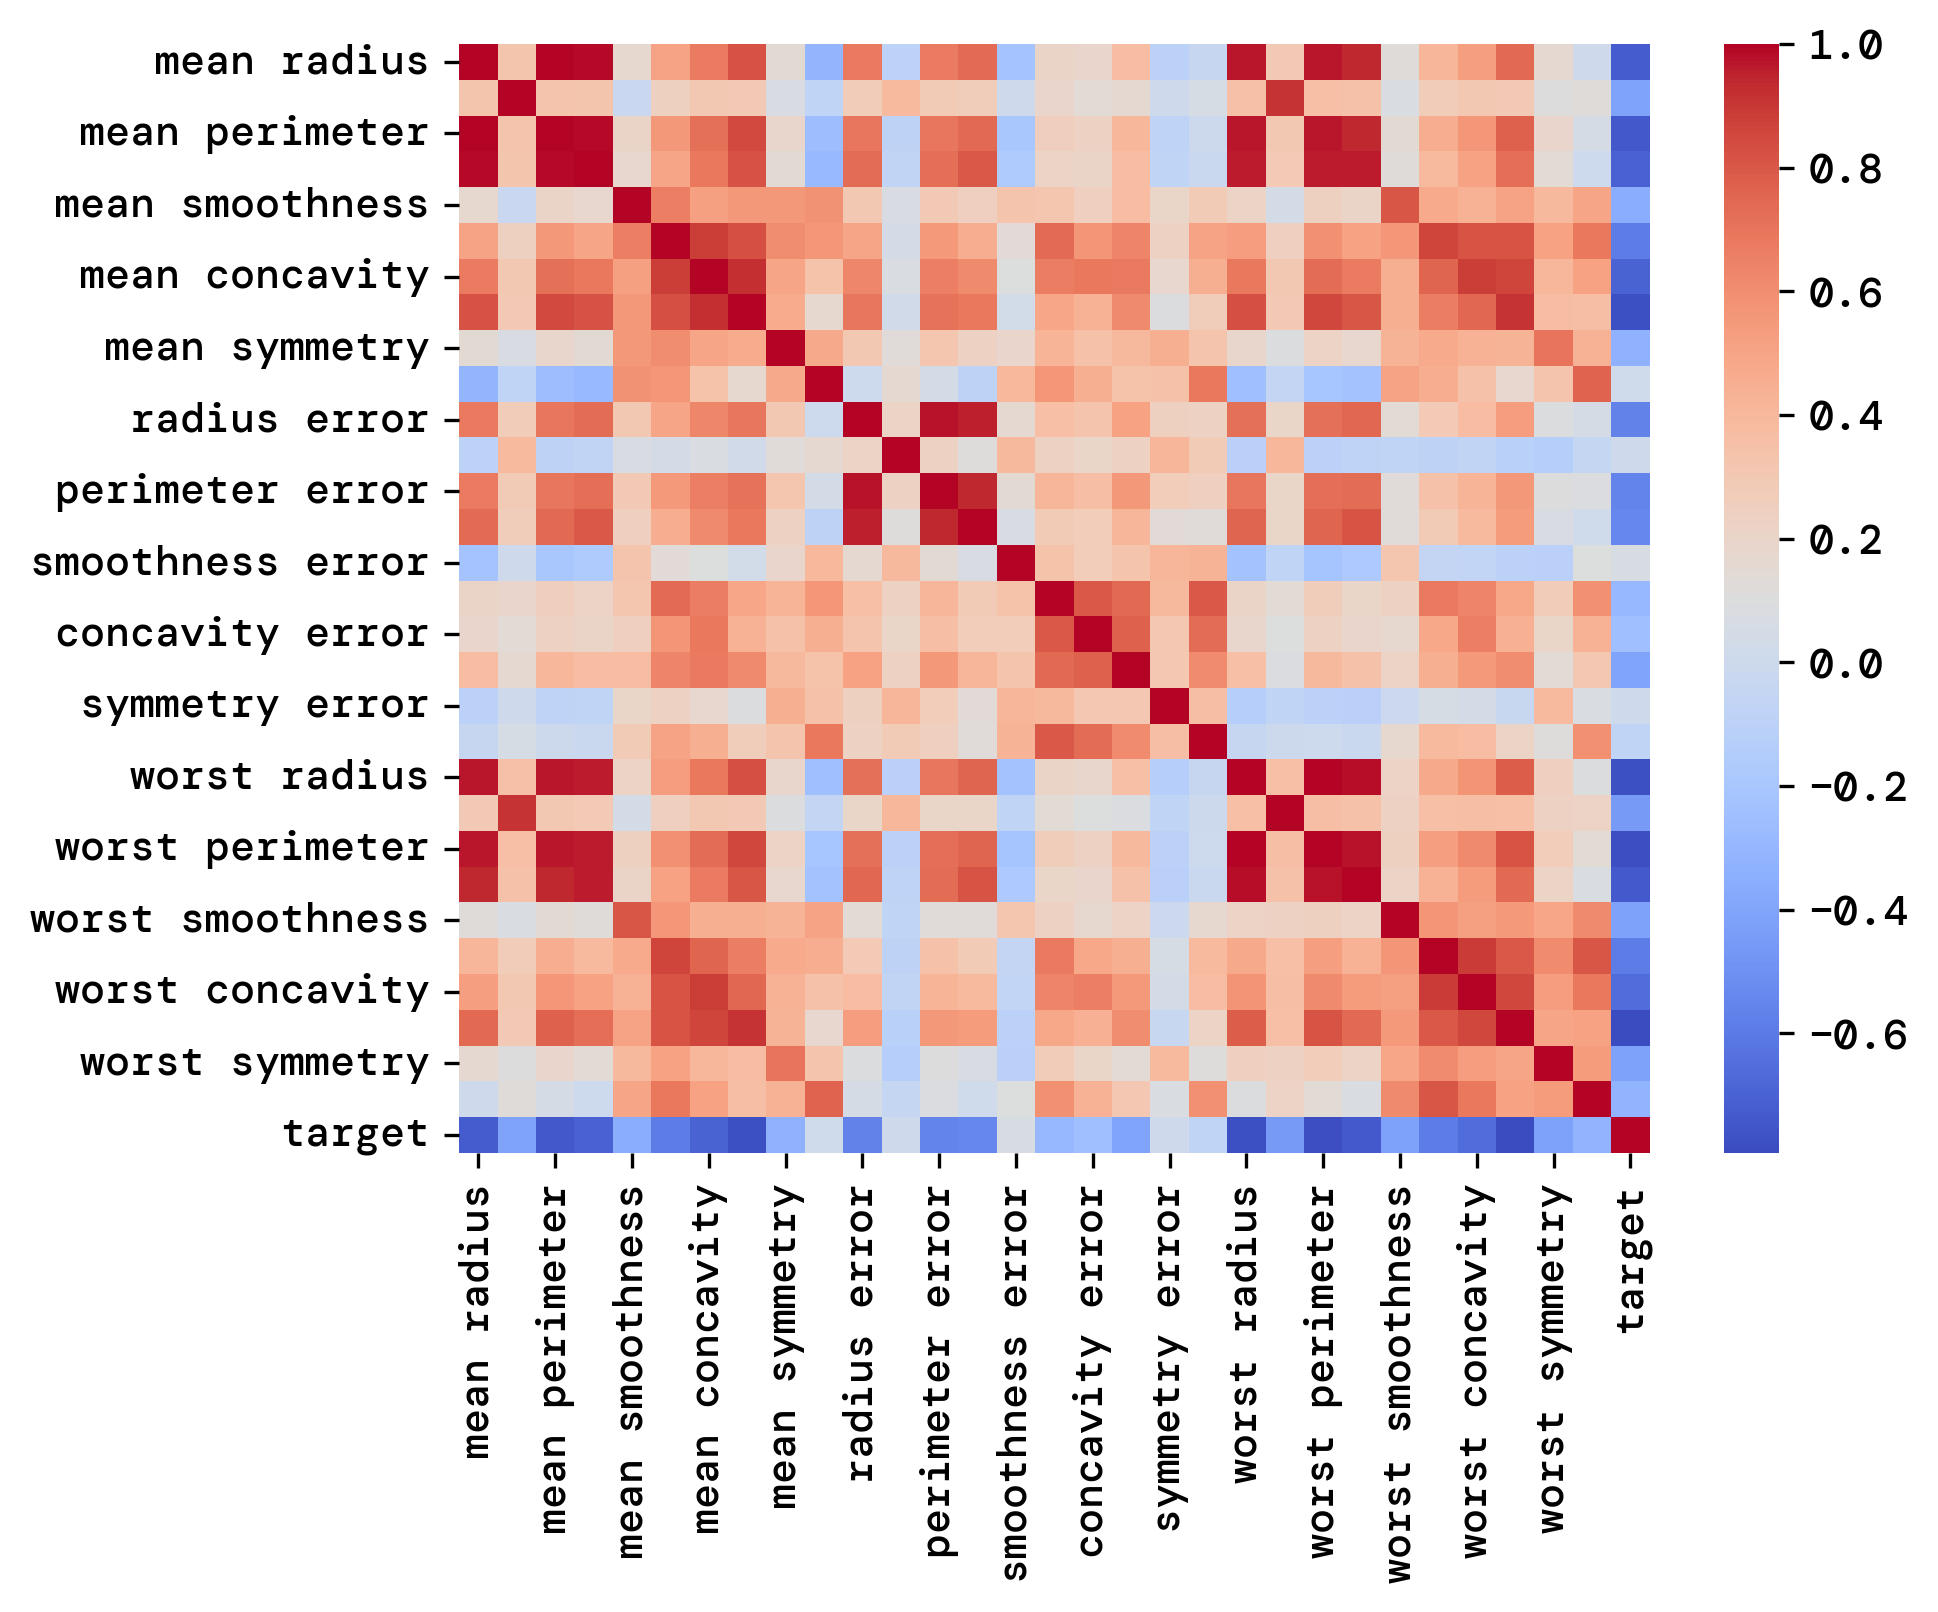
\includegraphics[width=0.8\textwidth]{../runsAndFigures/feature_correlation.png}
        \end{center}
        \caption{Feature correlation matrix. This provides insight into the redundancy among features. 
        Only every other feature is annotated, but the missing labels can be inferred from 
            Figure~\ref{fig:feature_histogram}.}\label{fig:feature_correlation}
    \end{figure}

    \begin{figure}
        \begin{center}
            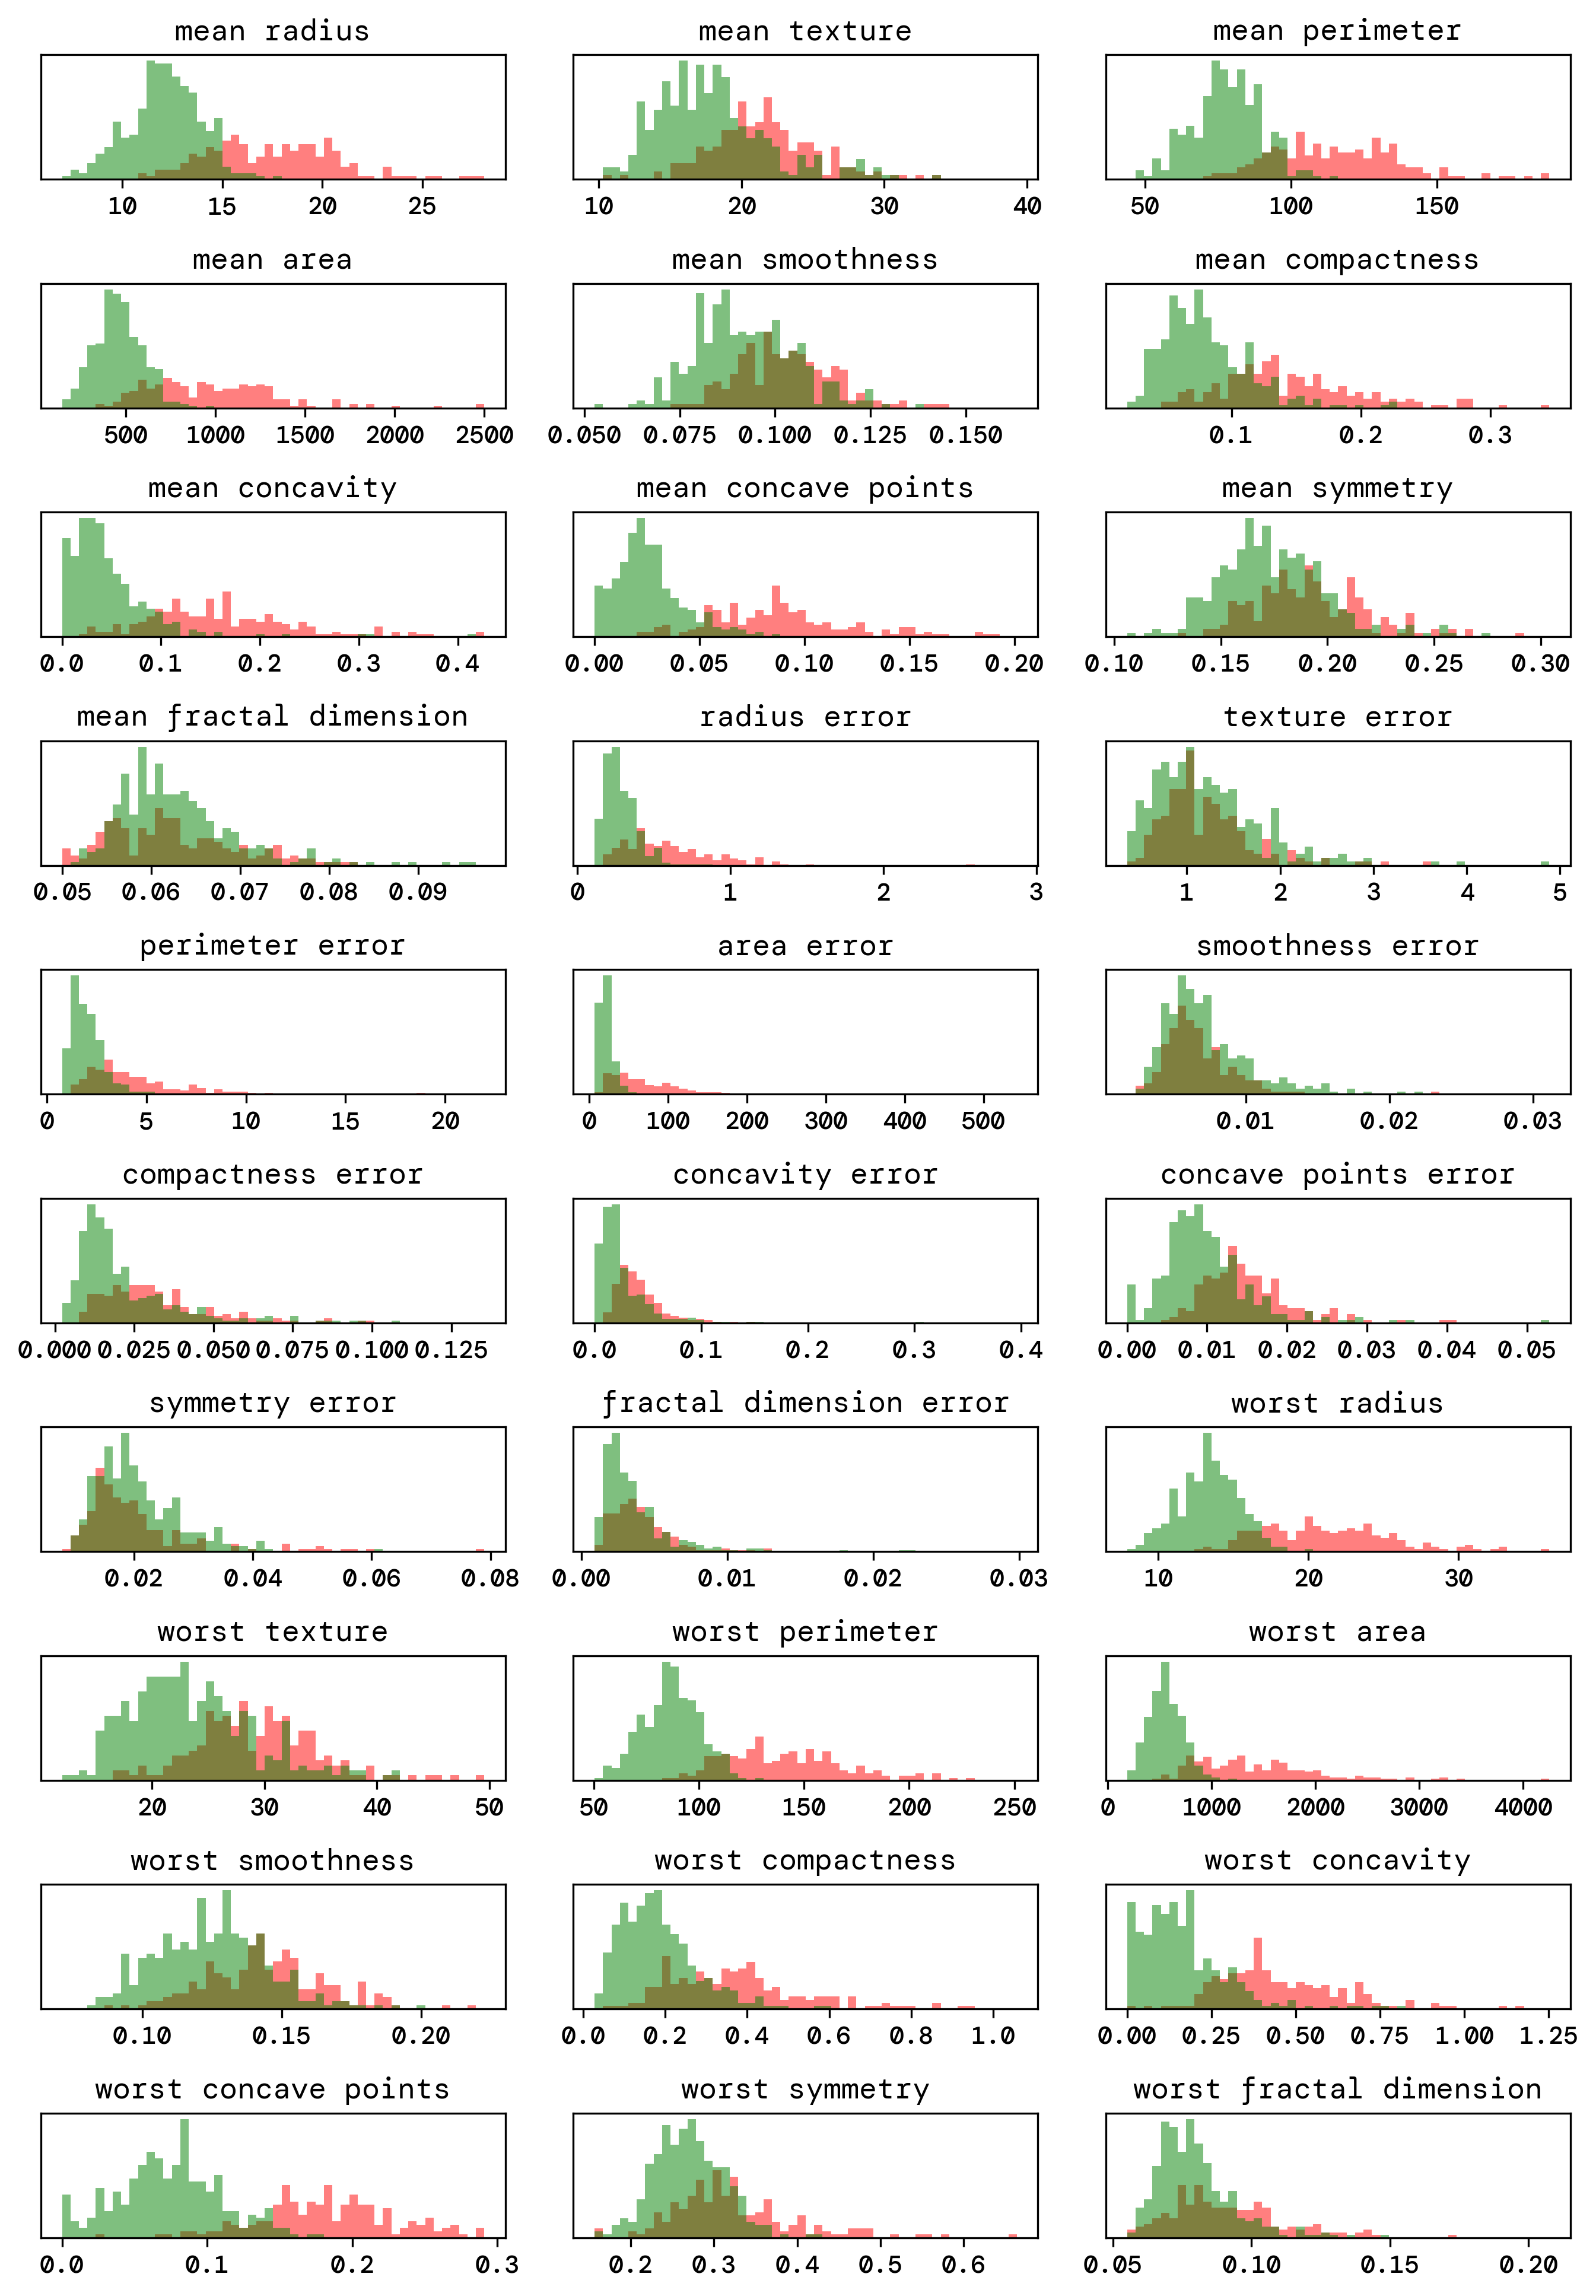
\includegraphics[width=0.95\textwidth]{../runsAndFigures/feature_histogram.png}
        \end{center}
        \caption{Feature histogram. The red class ($0$) represents malignant cases, while the green class 
        ($1$) indicates benign cases.}\label{fig:feature_histogram}
    \end{figure}


\clearpage

\section{Results and Analysis}
\label{sec:resultsdiscussion}

    In our experiments, we employed the cross-entropy loss function, The gradient of the loss function 
    with respect to the model's parameters was computed using automatic differentiation. 
    We used the SKLearn\cite{scikit-learn}
    library to perform cross-validation for a more robust evaluation of our models.
    We used k-fold cross-validation with $k=6$ folds. The results presented in this section are based on
    the average of the results from the 6 folds. The bar plots also show the standard deviation of the
    results from the 6 folds.


\subsection{Hyperparameters}
\label{sec:hyperparameters}

    During our hyperparameter tuning phase, we observed interdependencies between certain hyperparameters. Notably, 
    the learning rate and the number of epochs showed a significant correlation, as did the batch size and the learning 
    rate. Such dependencies imply that these hyperparameters cannot be optimized independently for the most effective 
    training process. Ideally, a comprehensive grid search across multiple dimensions of hyperparameters would be 
    conducted. However, due to constraints in time and computational resources, our experiments were limited.
    We were able to conduct grid searches, but these were restricted to two dimensions at most. While this limitation 
    prevented a thorough exploration of the hyperparameter space, the results from these partial grid searches provided 
    valuable insights. They served as indicators, pointing us towards regions in the hyperparameter space where optimal 
    settings might exist.
    The analysis of these results suggests that while we have identified promising hyperparameter settings, a more 
    exhaustive search might yield further improvements. 
    We use the same base hyperparameters when we tune the other hyperparameters.

    \begin{figure}[!ht]
        \begin{minipage}[t]{0.5\textwidth - 1mm}
            \begin{center}
                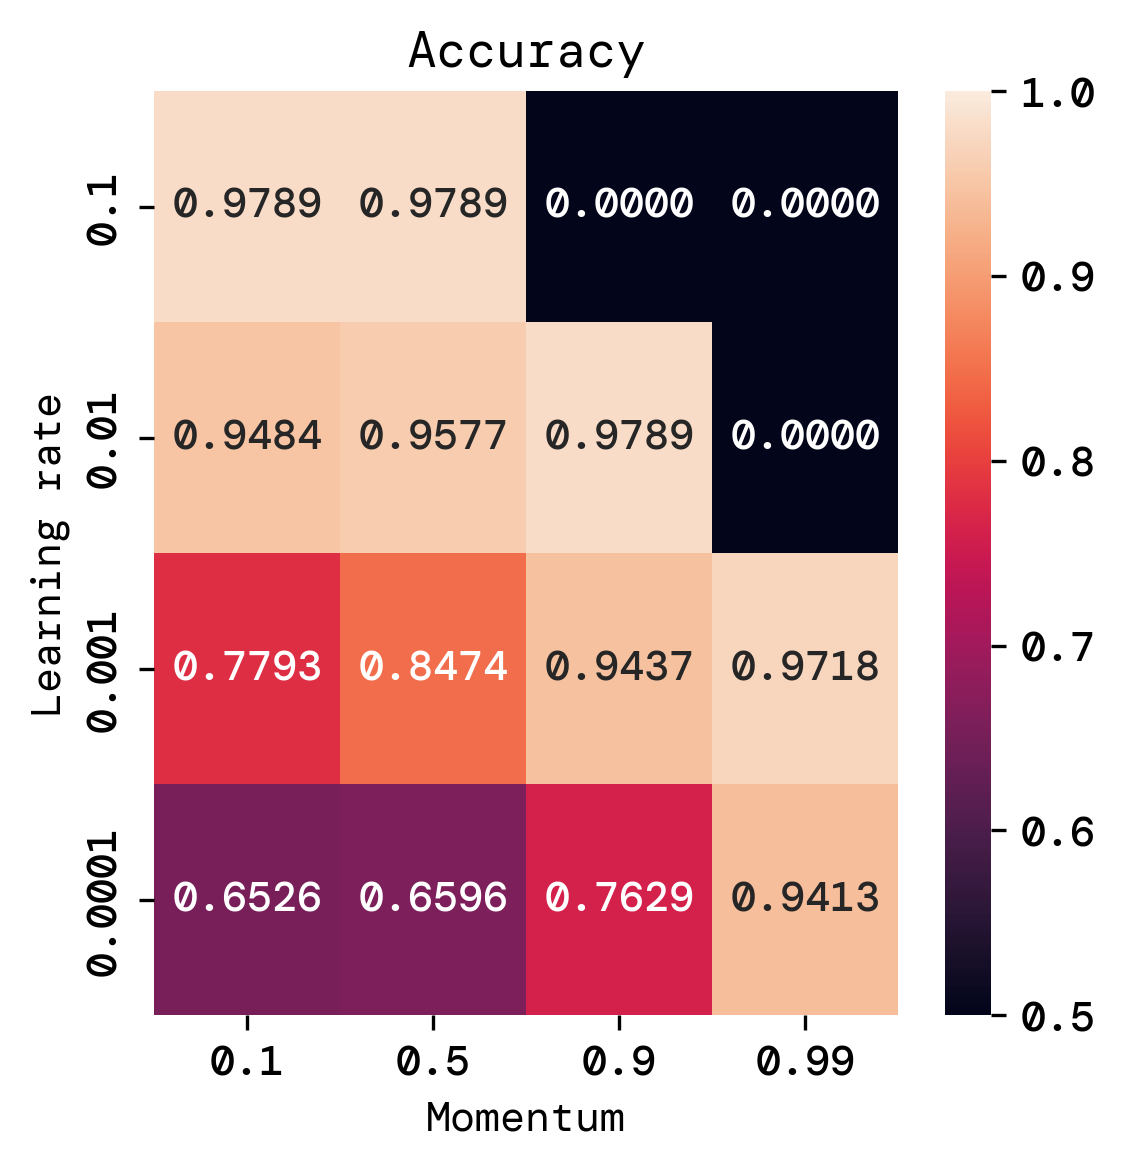
\includegraphics[width=\textwidth]{../runsAndFigures/accuracy_lr_gamma.png}
            \end{center}
            \caption
            {
                Accuracy versus learning rate and momentum.
            }\label{fig:accuracy_lr_gamma}
        \end{minipage}
        \hspace{2mm}
        \begin{minipage}[t]{0.5\textwidth - 1mm}
            \begin{center}
                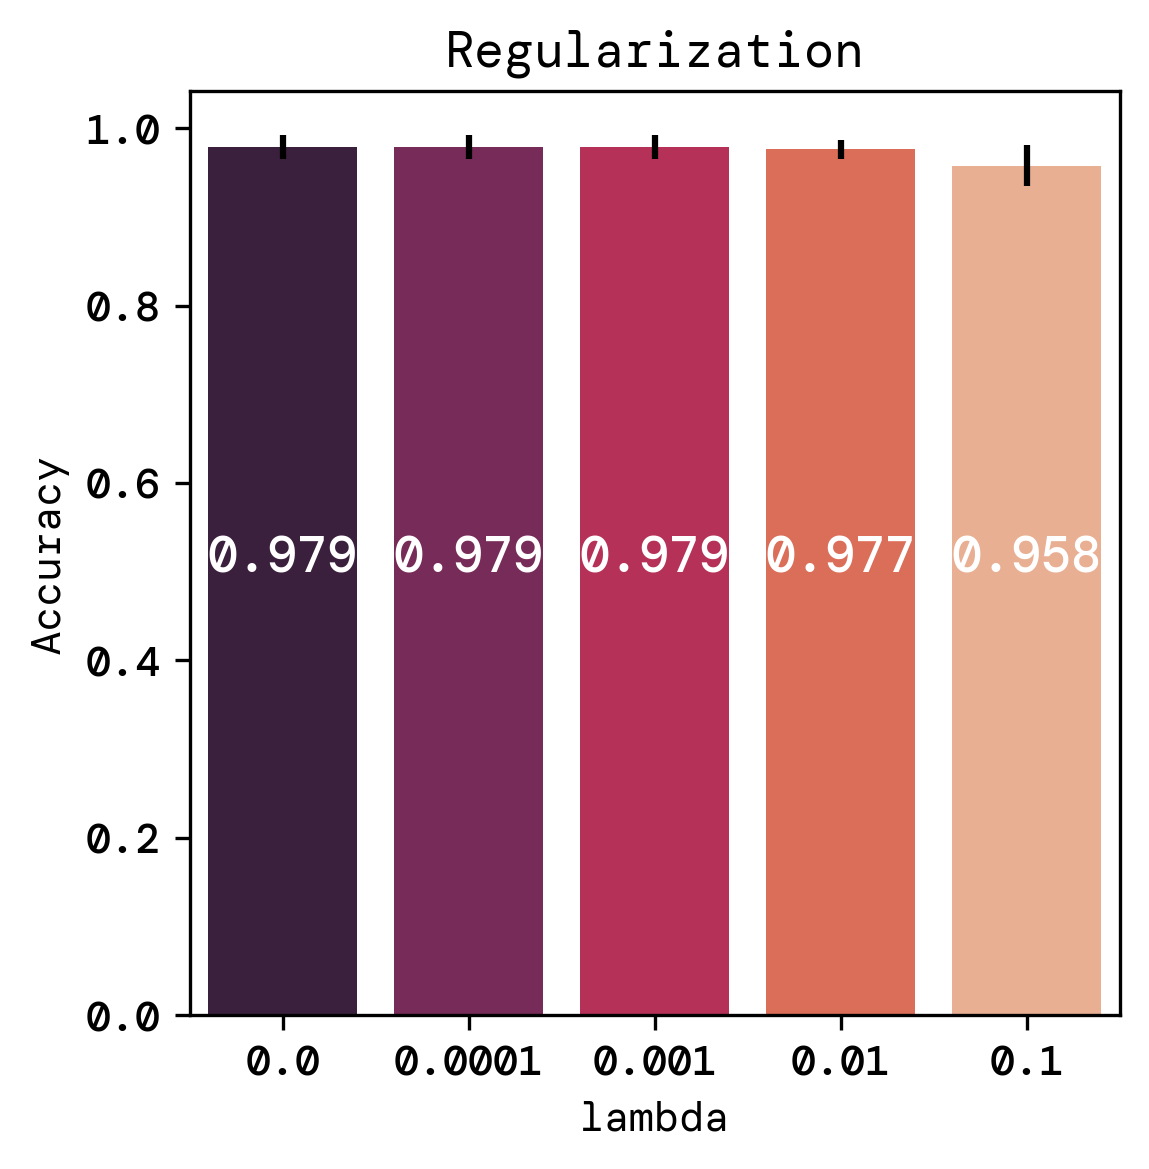
\includegraphics[width=\textwidth]{../runsAndFigures/accuracy_alpha.png}
            \end{center}
            \caption
            {
                Accuracy versus regualarization.
            }\label{fig:accuracy_aplha}
        \end{minipage}
    \end{figure}

    \noindent
    Our findings indicate that incorporating momentum is beneficial, particularly with a value of 
    around 0.9, which emerged as the most effective in our tests. This momentum allows for a higher learning rate, 
    enhancing the training process. In contrast, excessive regularization seems to adversely affect model performance.
    
    \begin{figure}[ht]
        \begin{minipage}[t]{0.5\textwidth - 1mm}
            \begin{center}
                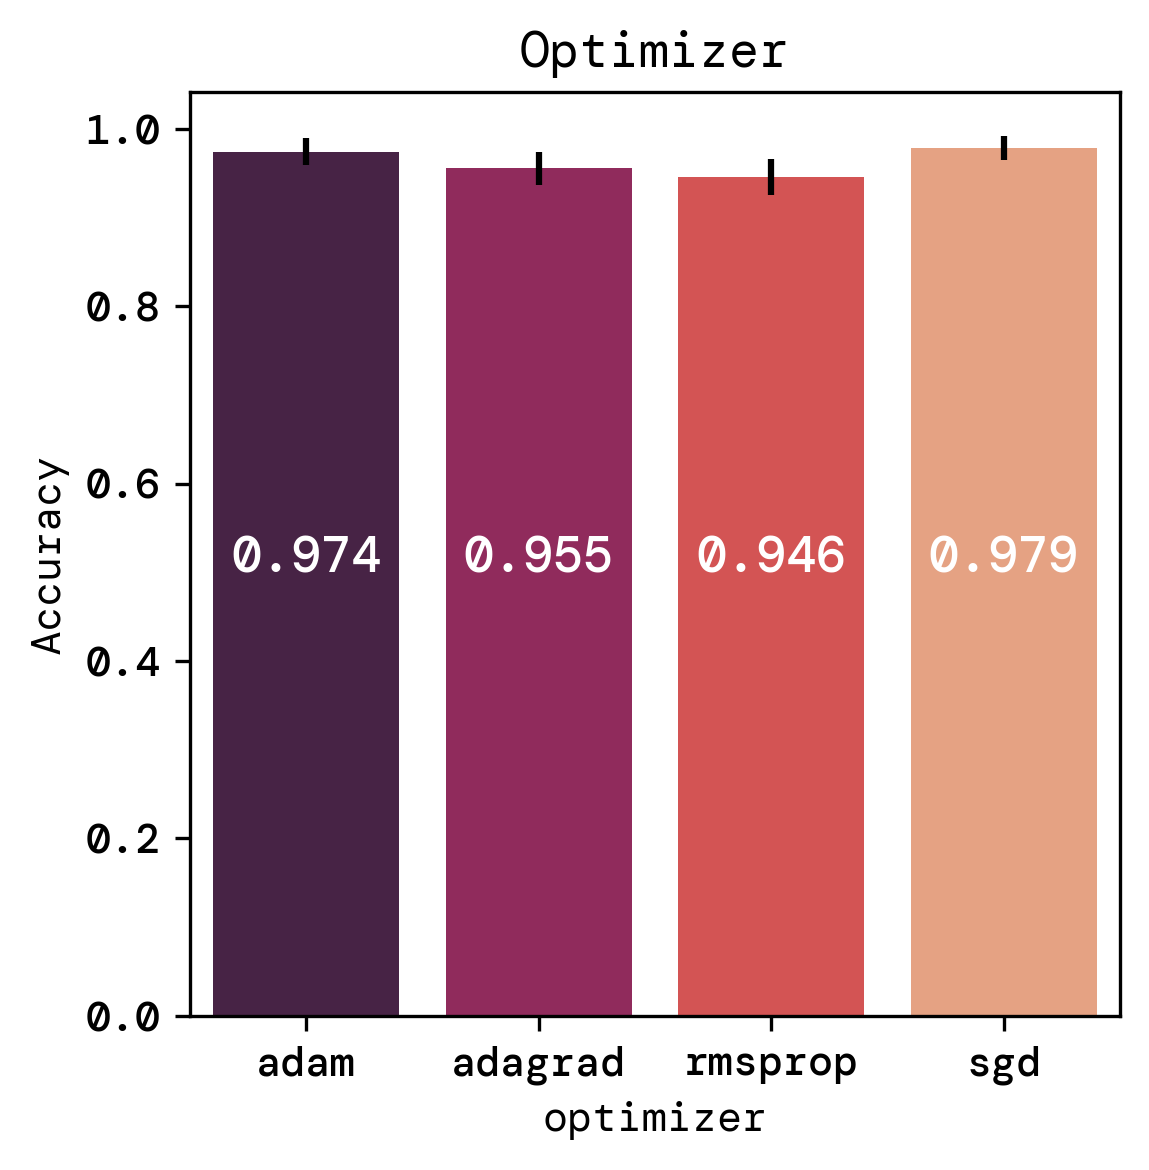
\includegraphics[width=\textwidth]{../runsAndFigures/accuracy_optimizer.png}
            \end{center}
            \caption
            {
                Model accuracy across different optimizers. here sgd is standard gradient descent.
            }\label{fig:accuracy_optimizer}
        \end{minipage}
        \hspace{2mm}
        \begin{minipage}[t]{0.5\textwidth - 1mm}
            \begin{center}
                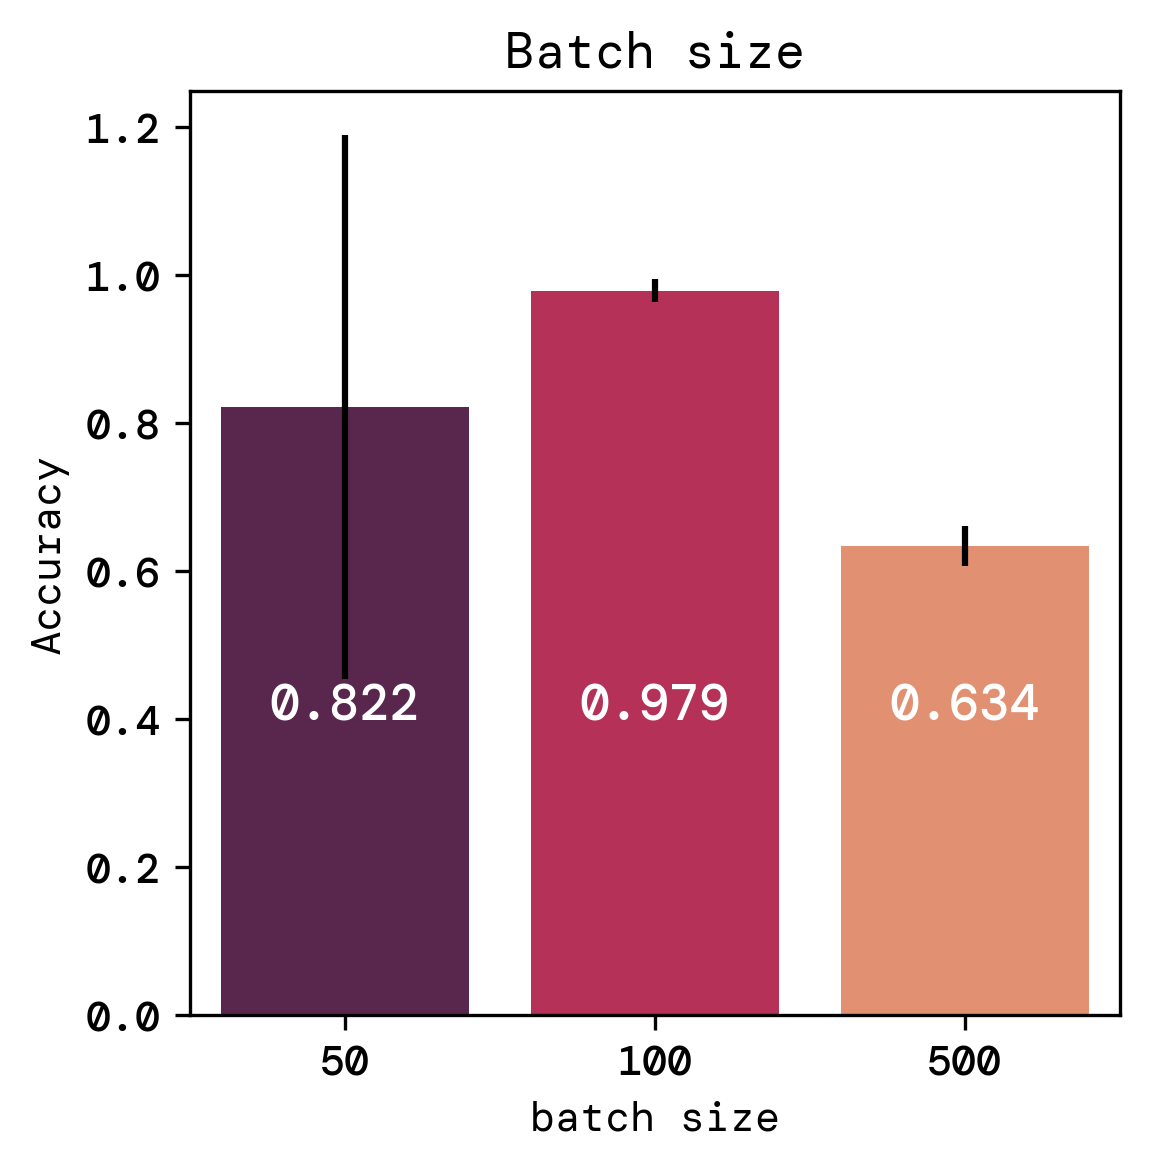
\includegraphics[width=\textwidth]{../runsAndFigures/accuracy_batch.png}
            \end{center}
            \caption
            {
                Accuracy based on batch size.
            }\label{fig:accuracy_batch}
        \end{minipage}
    \end{figure}

    \noindent
    The choice of optimizer did not significantly impact the model's performance. However, 
    Adam and standard gradient decent with momentum showed a slight advantage over others. 
    The batch size also played a role, with certain sizes yielding better accuracy. With a batch size of 50,
    the model accuracy varied greatly between folds.


    \begin{figure}[!ht]
        \begin{minipage}[t]{0.5\textwidth - 1mm}
            \begin{center}
                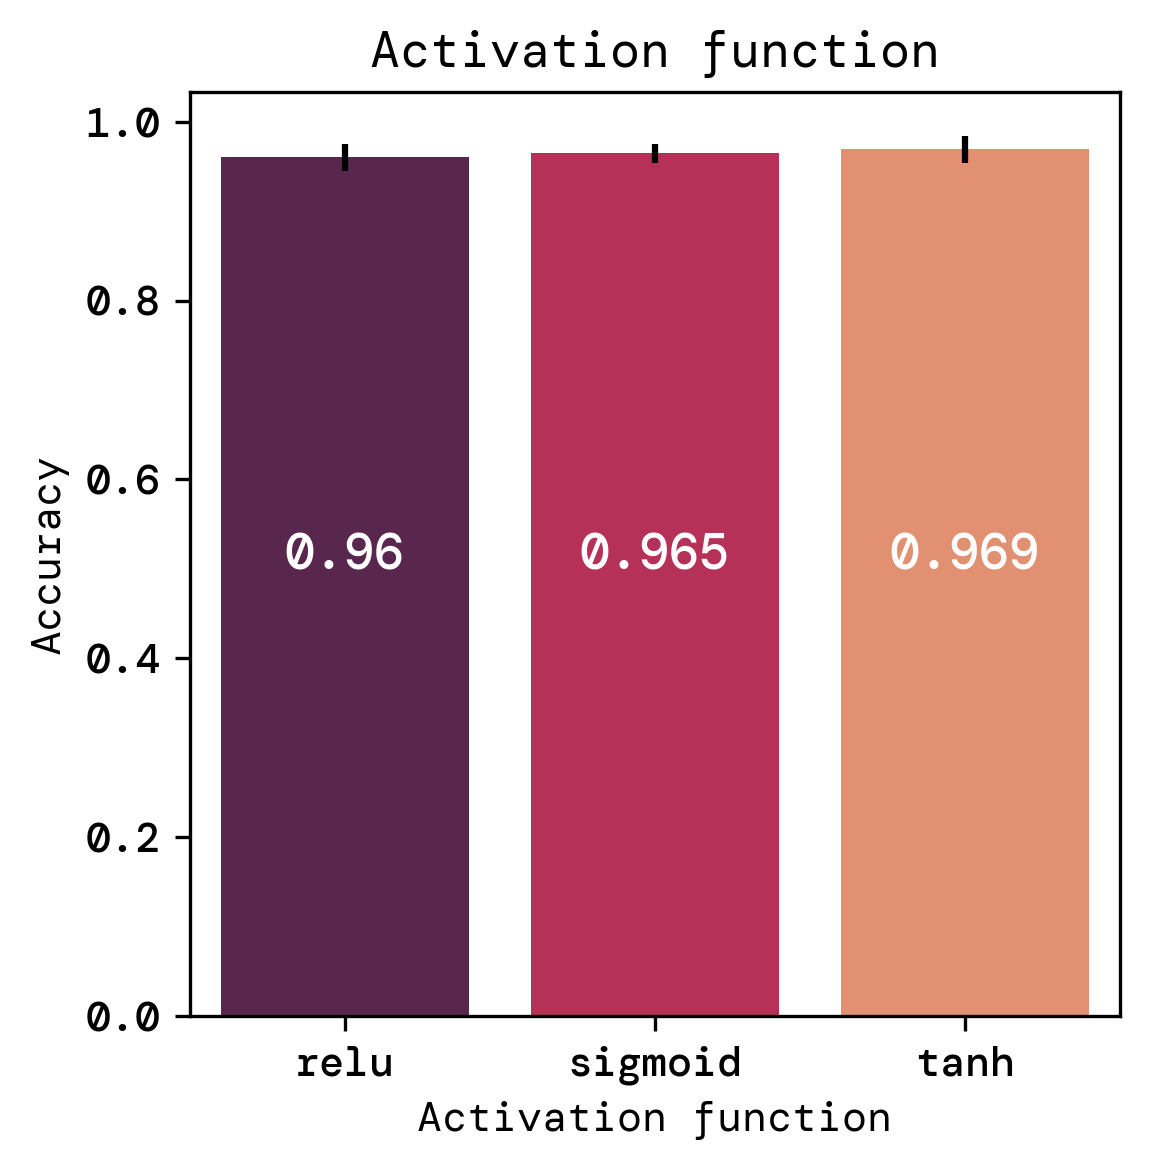
\includegraphics[width=\textwidth]{../runsAndFigures/accuracy_activ.png}
            \end{center}
            \caption
            {
                Model performance with different activation functions.
            }\label{fig:accuracy_activ}
        \end{minipage}
        \hspace{2mm}
        \begin{minipage}[t]{0.5\textwidth - 1mm}
            \begin{center}
                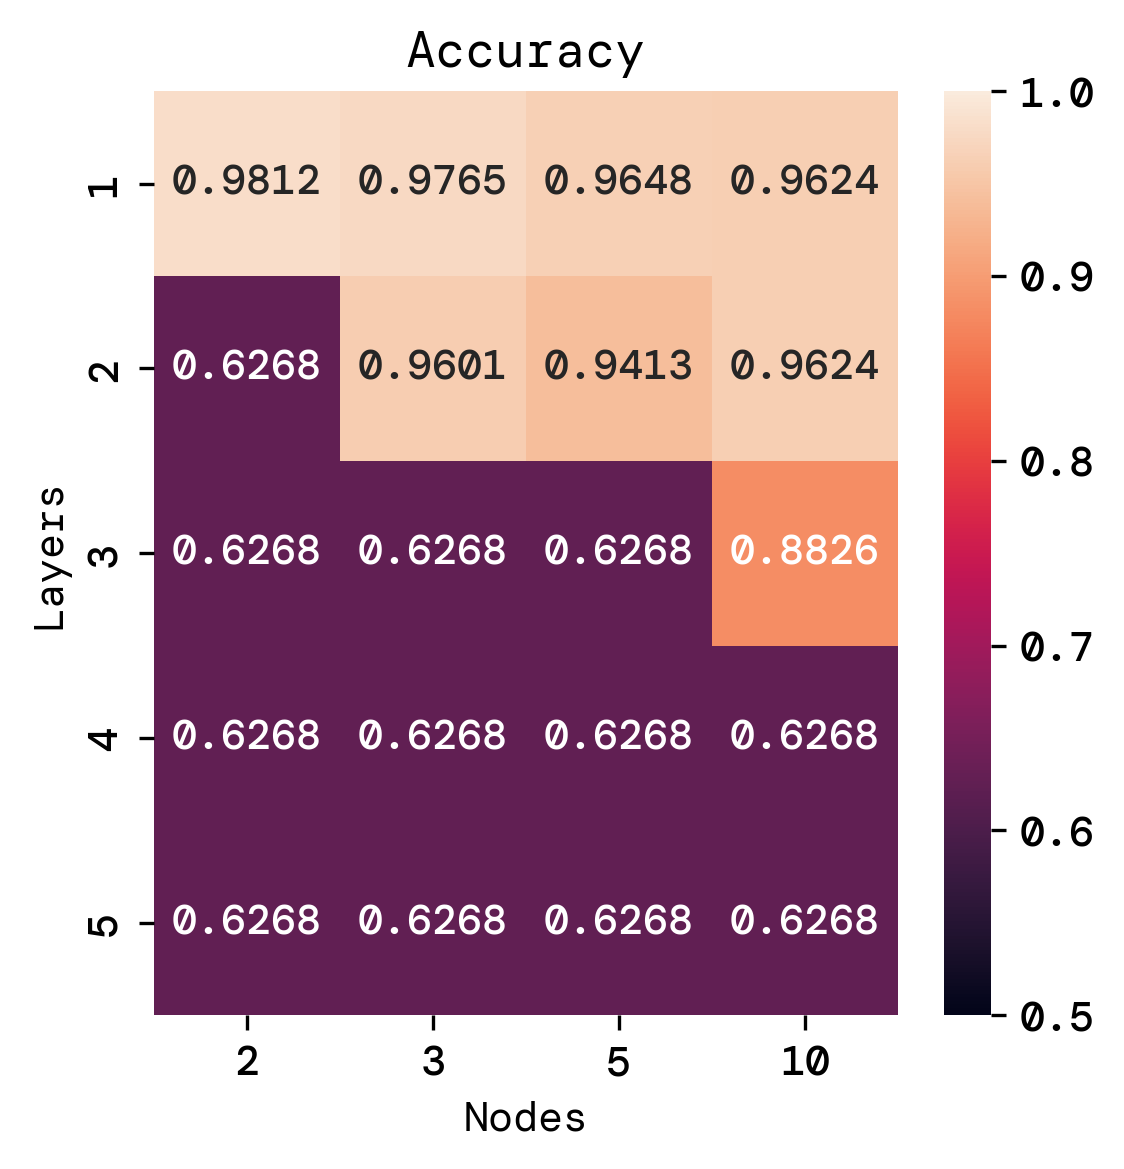
\includegraphics[width=\textwidth]{../runsAndFigures/accuracy_layers_nodes.png}
            \end{center}
            \caption
            {
                Accuracy in relation to the number of layers and nodes.
            }\label{fig:accuracy_layers_nodes}
        \end{minipage}
    \end{figure}


    \noindent
    \\
    In order for our model to correctly classify the data, it is essential that the last layer's activation function
    is a sigmoid function. This is because the sigmoid function outputs a value between 0 and 1, which can be
    interpreted as the probability of the data point belonging to class 1. The choice of activation function for the
    hidden layers did not significantly impact the model's performance.
    We used one hidden layer with 2 nodes when testing activation functions.

\newpage
\subsection{Final Evaluation and Comparisons}
\label{sec:comparisons}



    \begin{figure}[!ht]
        \begin{minipage}[t]{0.5\textwidth - 1mm}
            \begin{center}
                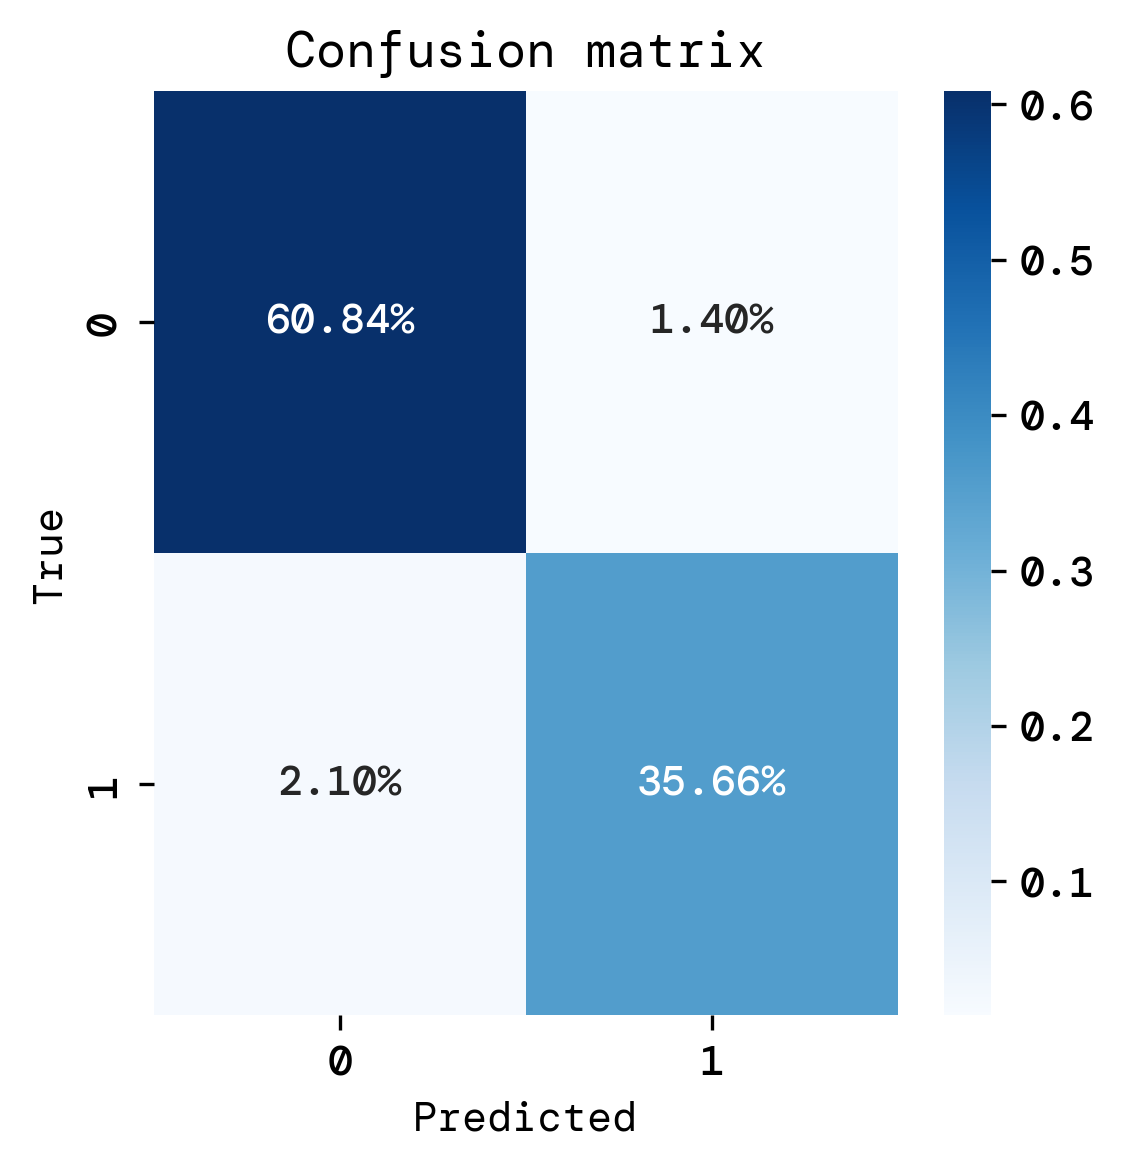
\includegraphics[width=\textwidth]{../runsAndFigures/confusion_matrix.png}
            \end{center}
            \caption
            {
                Confusion matrix for our model. 
            }\label{fig:confusion_matrix}
        \end{minipage}
        \hspace{2mm}
        \begin{minipage}[t]{0.5\textwidth - 1mm}
            \begin{center}
                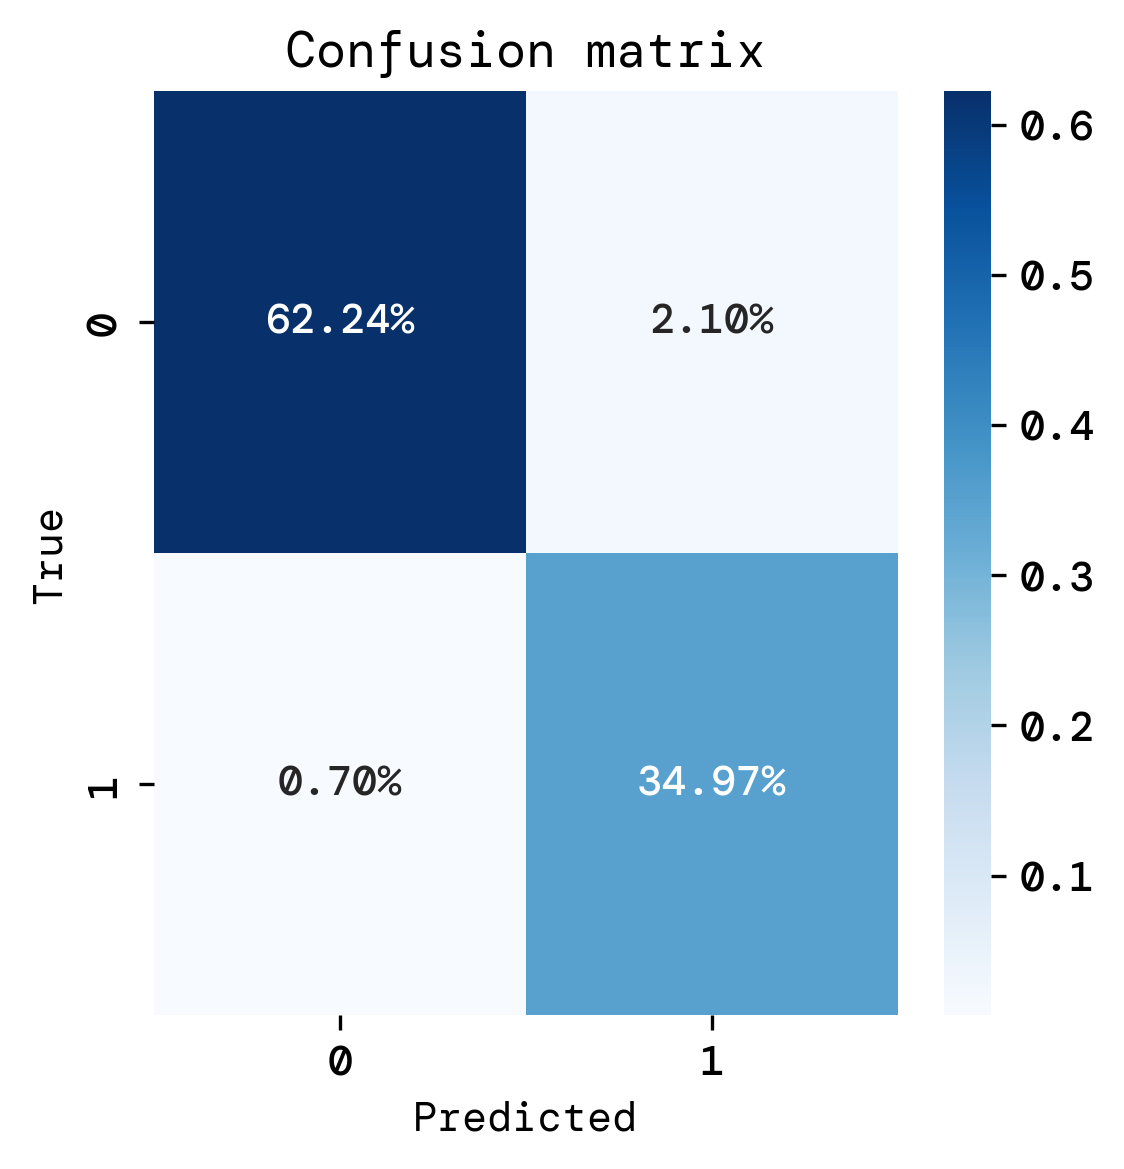
\includegraphics[width=\textwidth]{../runsAndFigures/confusion_matrix_sklearn.png}
            \end{center}
            \caption
            {
                Confusion matrix for SKLearn's model.
            }\label{fig:confusion_matrix_sklearn}
        \end{minipage}
    \end{figure}

    \noindent
    In our classification task, logistic regression achieved an accuracy of 96\% on the test set, 
    while our neural network model achieved 95\%. This performance is comparable to the 96\% accuracy 
    obtained with SKLearn's logistic regression model. It's important to consider that this comparison may not be 
    entirely direct due to differences in hyperparameters between the models. Nevertheless, efforts were made to 
    align the hyperparameters as closely as possible.
    An interesting observation is that increasing the number of layers and nodes in the neural network 
    did not significantly enhance its performance. This suggests the possibility of overfitting to the 
    training data, indicating that a simpler model could be more effective or that additional regularization 
    techniques might be required.
    
\section{Conclusion}
\label{sec:conclusion}

    
    This project has delved into the capabilities of neural networks in addressing classification challenges, 
    comparing them with traditional logistic regression models. Using the Wisconsin breast cancer dataset, we 
    found that neural networks, with a classification accuracy of 95\%, perform nearly as well as logistic regression 
    models, which achieved 96\%. This result is in line with the 97\% accuracy achieved using SKLearn's implementation.
    These findings highlight the competitive nature of neural networks in classification tasks, even when compared to 
    more traditional models. However, they also underscore the importance of careful model selection and hyperparameter 
    tuning in achieving optimal performance. While neural networks offer flexibility and power, they may not always 
    outperform simpler models, especially in cases where the underlying data patterns are not exceedingly complex.
    Future work could explore further optimization of the neural network architecture and hyperparameters, as well as 
    the application of these models to more diverse datasets to fully assess their generalizability and efficacy in 
    various classification scenarios.


    
    
     








% \acks{}


\clearpage 

\appendix
\renewcommand{\theHchapter}{appendix\Alph{chapter}}
\renewcommand{\theHsection}{appendix\thesection}

\phantomsection
\addcontentsline{toc}{chapter}{Appendix}


\chapter*{Appendix A}
\label{app:appendixA}




\vskip 0.2in
\bibliography{report}
% \bibliographystyle{apalike}
\bibliographystyle{plain}
\addcontentsline{toc}{section}{Bibliography}
\end{document}

